%%%% using 'arara' 4.0
% arara: xelatex: {synctex: yes, interaction: nonstopmode}
% arara: bibtex
% arara: xelatex: {synctex: yes, interaction: nonstopmode}
% arara: xelatex: {synctex: yes, interaction: nonstopmode}

%% arara: indent: {overwrite: yes}

% arara: clean: { extensions: [bcf, cod, blg, lof, lot, out, toc, xml, bak0 ] }

\documentclass[review]{elsarticle}

% Figures Links, mittig und rechts platzieren
\usepackage[export]{adjustbox}
\usepackage{caption}
\usepackage{subcaption}
\usepackage{amsmath}

\usepackage{enumerate}

% prevents that appendices are moved behind references
\usepackage{placeins}

\usepackage[nolist]{acronym}

\usepackage{longtable}
\usepackage{booktabs}
\usepackage{multirow}
\usepackage{float}

% https://tex.stackexchange.com/questions/165115/getting-not-defining-perthousnad-and-not-defining-micro-when-compiling-beamer
\usepackage{textcomp}

\graphicspath{{../03_figures/results/}{./}{../03_figures/data/}}

% enable linking to subsubsection
\setcounter{secnumdepth}{3}

% various symbols, e.g. \degree
\usepackage{gensymb}

\usepackage[hidelinks]{hyperref}

\usepackage{lineno}
\modulolinenumbers[5]

% set autoref abbr for appendix
\newcommand*{\Appendixautorefname}{appendix}

\journal{Journal "Remote Sensing of Environment"}

% line breaks in table cells
\newcommand{\specialcell}[2][l]{%
  \begin{tabular}[#1]{@{}l@{}}#2\end{tabular}}

% tilde
\newcommand{\mytilde}{\raise.17ex\hbox{$\scriptstyle\mathtt{\sim}$}}

%% APA style
\bibliographystyle{model5-names}\biboptions{authoryear}

\begin{document}

\begin{frontmatter}

	\title{Supporting ecological decision making using feature-selection and variable importance}
	%% Group authors per affiliation:
	\author[FSU]{Patrick Schratz}
	\cortext[mycorrespondingauthor]{Corresponding author}
	\ead{patrick.schratz@uni-jena.de}

	\author[FSU]{Jannes Muenchow}
	\author[NEIKER]{Eugenia Iturritxa}
	\author[LMU]{Bernd Bischl}
	\author[FSU]{Alexander Brenning}

	\address[FSU]{Department of Geography, GIScience group, Grietgasse 6, 07743, Jena, Germany}
	\address[NEIKER]{NEIKER, Granja Modelo –Arkaute, Apdo. 46, 01080 Vitoria-Gasteiz, Arab, Spain}
	\address[LMU]{Department of Statistics, Chair for computational Statistics, Ludwig-Maximilian University Munich, Germany}

	\begin{abstract}

	\end{abstract}

	\begin{keyword}
		hyperspectral imagery \sep forest health modeling \sep machine-learning \sep feature-selection  \sep model comparison
	\end{keyword}

\end{frontmatter}

\linenumbers

% längste Abkürzung steht hier!!! in eckigen Klammern
\begin{acronym}[AUROC]

	% geringerer Zeilenabstand
	%\setlength{\itemsep}{-\parsep}
	\acro{AGB}{above-ground biomass}
	\acro{ALS}{airborn laser scanning}
	\acro{ANN}{artificial neural network}
	\acro{AUROC}{area under the receiver operating characteristics curve}
	\acro{BRT}{boosted regression trees}
	\acro{CART}{classification and regression trees}
	\acro{CNN}{convolutional neural networks}
	\acro{CV}{cross-validation}
	\acro{DAP}{digital aerial photogrammetry}
	\acro{ENM}{environmental niche modeling}
	\acro{FPR}{false positive rate}
	\acro{FFS}{forward feature-selection}
	\acro{FS}{feature-selection}
	\acro{GAM}{generalized additive model}
	\acro{GBM}{gradient boosting machine}
	\acro{GLM}{generalized linear model}
	\acro{ICGC}{institut cartografic i geologic de catalunya}
	\acro{IQR}{interquartile range}
	\acro{MARS}{multivariate adaptive regression splines}
	\acro{MEM}{maximum entropy model}
	\acro{ML}{machine-learning}
	\acro{NDII}{normalized difference infrared index}
	\acro{NIR}{near-infrared}
	\acro{NRI}{normalized ratio index}
	\acro{OLS}{ordinary least squares}
	\acro{LiDAR}{light detection and ranging}
	\acro{LOWESS}{locally weighted scatter plot smoothing}
	\acro{PISR}{potential incoming solar radiation}
	\acro{PCA}{principal component analysis}
	\acro{PLS}{partial least-squares}
	\acro{RBF}{radial basis function}
	\acro{RF}{random forest}
	\acro{RMSE}{root mean square error}
	\acro{RR}{ridge regression}
	\acro{RSS}{residual sum of squares}
	\acro{SAR}{synthetic aperture radar}
	\acro{SDM}{species distribution modeling}
	\acro{SMBO}{sequential-based model optimization}
	\acro{SVM}{support vector machine}
	\acro{TPR}{true positive rate}
	\acro{VI}{vegetation index}
	\acro{XGBOOST}{extreme gradient boosting}
\end{acronym}

\section{Introduction}
\label{sec:intro}

% Explain how remote sensing is used in forestry (potential to map forest health)
% Link remote sensing and machine-learning
\noindent The use of \ac{ML} algorithms for analyzing remote sensing data has seen a huge increase in the last decade \citep{lary2016}.
Especially since the launch of the first Sentinel satellite in 2014 the amount of freely available imagery data has increased greatly.
At the same time, the implementation and usability of algorithms (both statistical and machine-learning) has been greatly simplified in the open-source community.
Scientists can nowadays relatively easily feed large amounts of information into complex models in a semi-automated way.
These points enable the possibility to analyze (temporal) changes of the environment on a large scale \citep{ma2015}.

% link to forest health analysis and show exemplary studies
Machine-learning methods in combination with remote-sensing data are used in many environmental fields such as vegetation cover analysis or forest carbon storage mapping \citep{mascaro2014, urban2018}.
The advantages of conducting analysis at large scale make these points a promising toolset also for forest health analysis.
This research field aims to enhance the understanding of biotic and abiotic triggers, for example by analyzing defoliation at trees \citep{hawrylo2018}.
Different approaches exist including temporal change detections \citep{zhang2016} or analysis about the current health status of forests on a stand level \citep{townsend2012}.
Defoliation at trees is an information which is able to serve as a proxy for forest health by describing the impact of biotic and abiotic pest triggers \citep{townsend2012, goodbody2018}.
Vegetation indices have shown the potential to provide valuable information when analyzing such scenarios \citep{jiang2014, adamczyk2015}.
Since both triggers and tree types are highly variable across regions, it cannot be known apriori which indices are most important for describing the actual relationship.
This emphasizes the need to extract as much information as possible from the available input data to generate features that can possibly explain the modeled relationship.
Besides \ac{VI} a less known type of indices that can be calculated from remote-sensing products are \ac{NRI}.
\ac{NRI} are arbitrary combinations of band information from remote-sensing data.
Especially when working with hyperspectral data, \ac{NRI} provide the possibility to calculate hundreds of indices that can be used during modeling.

% now that we introduced the importance of remote sensing indices for forest health,

Despite its popularity in environmental modeling, there are no studies so far that used machine-learning algorithms in combination with remote-sensing data to analyze defoliation on a tree level.
This study aims at closing this gap by analyzing defoliation at trees in northern Spain using airborne hyperspectral data.
To cope with the state-of-the-art methodology in modeling, a methodology which combines feature-selection and hyperparameter tuning across multiple algorithms is used.
The approach of generating many features comes along with the introduction of "high-dimensionality" into the analysis \citep{trunk1979, xu2016}.
Even though \ac{ML} algorithms are capable of handling highly-correlated input variables, the fitting time of models increase substantially and the interpretation of results becomes more complicated.
Besides modeling defoliation at trees this work also aims at providing an exemplary analysis of how to deal with spatial feature-rich data derived from a hyperspectral remote-sensing source.

The reseach questions of this study are the following:

\begin{itemize}
	\item Do different environmental feature sets show substantial differences in performance when predicting defoliation at trees?
	\item How are different feature-selection methods performing and do they improve the predictive performance of the final model?
	\item Is it possible to map defoliation at a tree level using high-resolution hyperspectral data at a sufficient error rate?
	\item Which features were most important to the model to detect defoliation at trees?\end{itemize}

\noindent State-of-the-art machine-learning techniques were compared using three feature sets with different feature-selection approaches including a relatively novel approach of ensemble filters.
Model-based optimization was applied for hyperparameter tuning of the chosen algorithms.
Spatial block \ac{CV} was used to account for spatial autocorrelation in the data.

\section{Data and study area}
\noindent Airborne hyperspectral data with a spatial resolution of one meter and 126 spectral bands was available for four Monterey Pine (\textit{Pinus radiata}) plantations in northern Spain.
The trees in the study area plots suffer from infections of invasive pathogens such as \textit{Diplodia sapinea}, \textit{Fusarium circinatum}, \textit{Armillaria mellea} or \textit{Heterobasidion annosum} leading to a spread of cankers or defoliation \citep{mesanza2016, iturritxa2017}.
In-situ measurements of defoliation at trees (as a proxy for tree health) were collected to serve as the response variable \textit{defoliation} spanning a range from 0\% - 100\% (\autoref{fig:defol-distr}).
The fungi are assumed to infect the trees through open wounds, possibly caused by previous hail damage \citep{iturritxa2014}.
The dieback of these trees, which are mainly used as timber, causes high economic damages \citep{ganley2009}.

\begin{figure} [t!]
	\begin{center}
		\makebox[\textwidth]{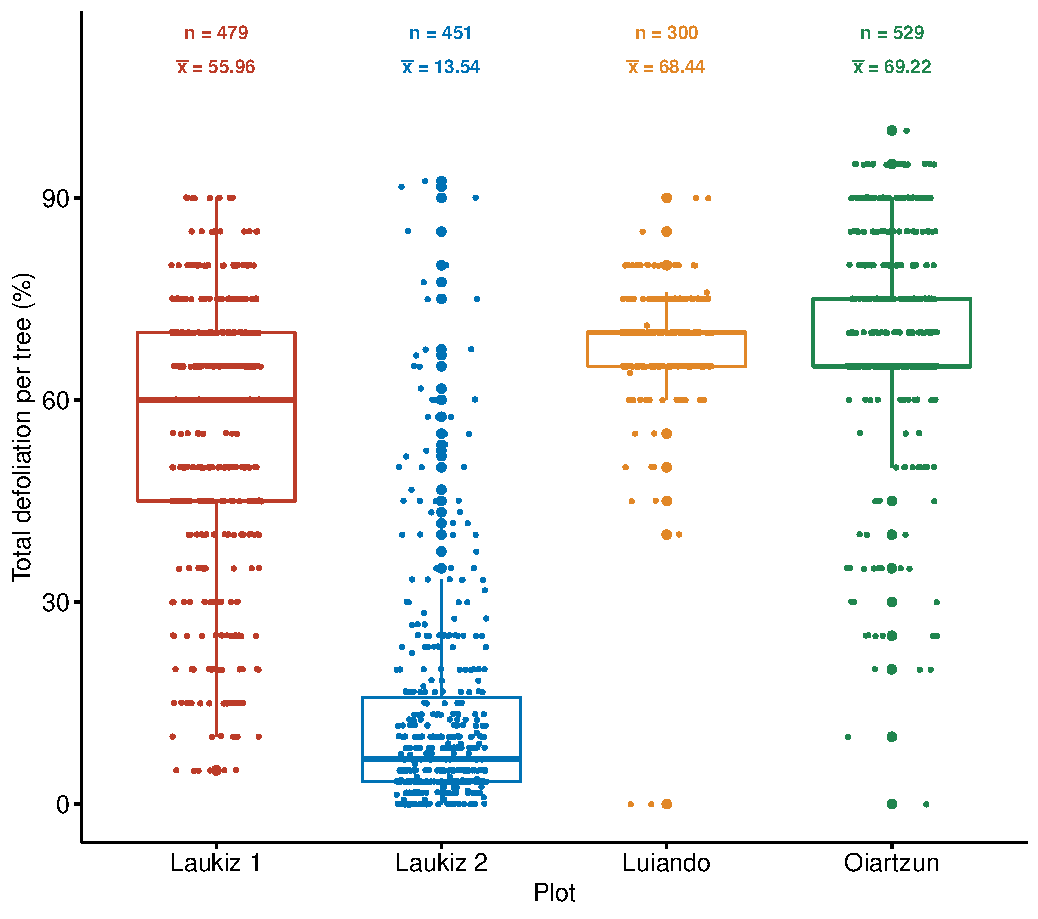
\includegraphics[width=0.7\textwidth] {defoliation-distribution-plot-1.pdf}}
		\caption{Distribution of defoliation at trees for plots Laukiz 1, Laukiz 2, Luiando and Oiartzun.}
		\label{fig:defol-distr}
	\end{center}
\end{figure}



\subsection{In-situ data}

\noindent The \textit{Pinus radiata} plots of this study, namely \textit{Laukiz 1}, \textit{Laukiz 2}, \textit{Luiando} and \textit{Oiartzun}, are located in the northern part of the Basque Country (\autoref{fig:study_area}).
\textit{Oiartzun} has the most observations (n = 529) while \textit{Laukiz 2} features the largest area size (1.44 ha).
All plots besides \textit{Luiando} are located nearby the coast (\autoref{fig:study_area}).
In total 1759 observations are available (\textit{Laukiz 1} = 479, \textit{Laukiz 2} = 451, \textit{Luiando} = 300, \textit{Oiartzun} = 529).
The data was surveyed in September 2016.

\begin{figure} [t!]
	\begin{center}
		\makebox[\textwidth]{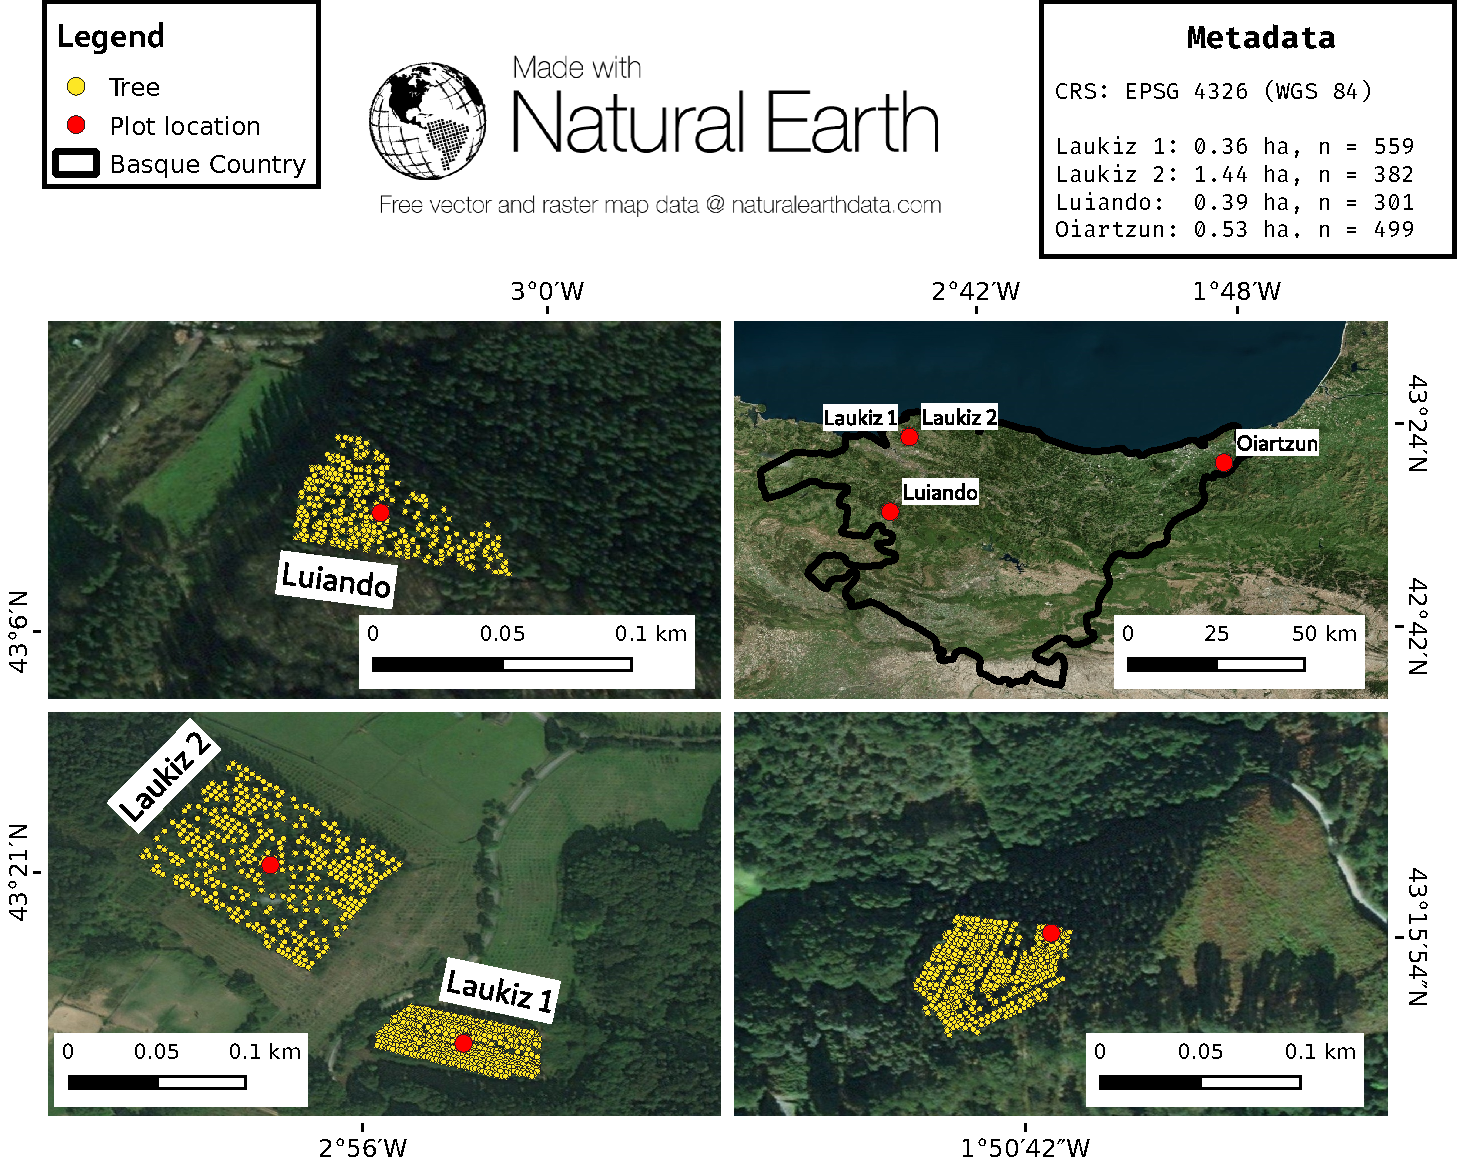
\includegraphics[width=\textwidth] {study_area_hyperspectral.pdf}}
		\caption{Information about location, size and spatial distribution of trees for all plots used in this study.}
		\label{fig:study_area}
	\end{center}
\end{figure}


\subsection{Hyperspectral data}

\noindent The airborne hyperspectral data was acquired during two flight campaigns on September 28th and October 5th 2016, both around 12 am.
The images were taken using a AISAEAGLE-II sensor.
All preprocessing steps (geometric, radiometric, atmospheric) have been conducted by the \ac{ICGC}.
The first four bands are corrupted, leaving 122 bands with valid information.
Additional metadata information is available in \autoref{tab:hyperparameter_limits}.

% parameter limits
\begin{table}[b!]
\centering
\caption[t]{Specifications of hyperspectral data.}
\begingroup\footnotesize
\begin{tabular}{ll}
	\\
	Characteristic         & Value                               \\
	\hline
	Geometric resolution   & 1 m                                 \\
	Radiometric resolution & 12 bit                              \\
	Spectral resolution    & 126 bands (404.08 nm - 996.31 nm)   \\
	Correction:            & Radiometric, geometric, atmospheric
\end{tabular}
\endgroup
\label{tab:hyperparameter_limits}
\end{table}

\section{Methods}

\subsection{Derivation of indices}
% TODO: Mention different feature sets
\noindent To use the full information from the hyperspectral data, all possible vegetation indices supported by the R package \textit{hsdar} (90 in total) as well as all possible \ac{NRI} combinations were calculated.
The following formula was used for the NRI calculation:

\begin{equation}
	NRI_{i,j} = \frac{b_{i} - b_{j}}{b_{i} + b_{j}}
\end{equation}

\noindent
where $i$ and $j$ are the respective band numbers.

\bigbreak

\noindent To account for geometric offsets (which were reported with up to 1 m from \ac{ICGC}), a buffer of two meters around the centroid of the respective tree was drawn.
The value assigned to a tree observations was the mean of all pixels which touched the respective buffer around the tree.
In total, $\frac{125*126}{2} = 7875$ NRIs were calculated .
Due to four corrupted bands of the sensor a total of 7471 indices were available for each observation.

\subsection{Dimension reduction}

\noindent It is important to distinguish the term "dimension reduction" from "high-dimensionality".
The former refers to the general idea of reducing features from a dataset \citep{vandermaaten2007}.
In modeling this means finding the best subset of covariates which provide the most predictive power to the model or extracting the main components of the features using a \ac{PCA}.
"High-dimensionality" in contrast is defined as a dataset attribute and applies when $p > n,$ where $p$ is the number of covariates and $n$ the number of observations \citep{hastie2001}.
There is no absolute value at which the term can be applied, both for $n$ and $p$.
Hence for this study the word "high-dimensionality" only applies to the experiments using the "NRI" feature set (7470 features for 1759 observations).

The case of a feature-rich dataset comes with several challenges for both model fitting and evaluation.

\begin{itemize}
  \item Model fitting times increase
  \item Noise is possibly introduced into models by highly-correlated variables \citep{johnstoneiainm.2009}
  \item Model interpretation and prediction tasks become more complicated \citep{johnstoneiainm.2009}
\end{itemize}

\noindent In the following sections a brief overview about sub-categories of feature-selection approaches is given.
Due to the focus of this study on the use of filter methods, all other appraoches were grouped into a single section.

\subsubsection{Filter methods}

% Filter methods
\noindent The concept of "Filter methods" originates on the idea of ranking features using certain heuristics of an algorithm \citep{chandrashekar2014}.
Some filter methods are restricted towards specific types of variables (numeric or nominal data).
After the covariates have been ranked, a decision needs to be made what features to keep and which to discard \citep{drotar2015}.
This step is usually done within the optimization phase of the model fitting, along with the hyperparameter tuning.
Essentially, the number of covariates in the model is treated as a hyperparameter of the model.
The goal is to optimize the number of features (using the ranked covariates) at which the model achieves the best performance.
In well-implemented software solutions the filter calculation is only done once and then cached, saving valuable resources \citep{mlr}.

\paragraph{Ensemble filter methods}

% Ensemble filter methods
Besides the concept of choosing a specific filter method to rank variables, studies showed that combining several filters using statistical operations such as "minimum", "mean" or "sum" are able to enhance the predictive performance of the resulting models \citep{abeel2010, drotar2017a}.
This approach is referred to as "ensemble filter" \citep{dietterich2000}.
Ensemble filters align with the recent rise of the "ensemble" approach in machine-learning which uses stacking to combine the predictions of multiple models, aiming to enhence predictive performance \citep{polikar2012, feurer2015}.
In this work the "Borda" ensemble filter was applied \citep{drotar2017a}.
The final order is the sum of all single filters ranking.

\paragraph{Ensuring a fair weighting in the ensemble}

Filter methods can be grouped into classes: Correlation based, entropy based, linear and non-linear methods.
It is important to not give certain classes too much weight in the ensemble as otherwise the final result will be biased.
This was taken care of by calculating the rank correlations (Spearman's correlation) of the generated feature rankings of all methods against each other.
In case filters showed high correlations with each other, these were not included into the ensemble filter.
This ensures that the ensembe filter is not biased towards a certain group of methods yielding highly similar rankings.

\paragraph{Description of used filter methods}

Filter methods can be classified as follows:

\begin{itemize}
	\item univariate/multivariate (scoring based on a single variable / multiple variables)
	\item linear/non-linear (calculation of linear/non-linear interaction terms)
	\item entropy/correlation (scoring based on derivations of entropy or correlation based approaches)
\end{itemize}

% filter methods
\begin{table}[b!]
\centering
\caption[t]{List of filter methods used in this work}
\begingroup\footnotesize
\begin{tabular}{lll}
	\\
	Name                                         & Group                             & Reference          \\
	\hline
	Linear correlation (Pearson)                 & univariate, linear, correlation   & \cite{pearson1901} \\
	Information gain                             & univariate, non-linear, entropy   & \cite{quinlan1986} \\
	Minimum redundancy, maximum relevance        & multivariate, non-linear, entropy & \cite{zhao2013}    \\
	Carscore                                     & multivariate, linear, correlation & \cite{zuber2011}   \\
	Relief                                       & multivariate, linear, entropy,    & \cite{kira1992}    \\
	Conditional minimal information maximization & multivariate, linear, entropy     & \cite{fleuret2004}
\end{tabular}
\endgroup
\label{tab:filter-methods}
\end{table}

\noindent Filter method "information gain" is by creation only defined for class responses:

\begin{equation}
	H(Class) + H(Attribute) - H(Class, Attribute)
\end{equation}

where $H$ is the conditional entropy of the response variable (class) or the feature (attribute), respectively.
To be able to use this method with a numeric response, the variable is discretized into equal bins and treated as a class variable.
While the number of bins can be treated as a hyperparameter of the filter method, the default of the R package implementation of \texttt{$n_{bin}$ = 5} was used after rank correlations of > 0.9 for different bin sizes have been explored.
% TODO: Add reference to appendix, put plot into appendix

\subsubsection{Wrapper methods and PCA}

\noindent Other approaches to assess feature importance are "wrapper methods" and the \ac{PCA} \citep{das2001, jolliffe2016}.
A short introduction to both is given below.

% Wrapper approach
\noindent "Wrapper methods" \citep{chandrashekar2014, kohavi1997} apply algorithms that are used for hyperparameter optimization such as "Random Search" or "Generic Simulated Annealing".
First a (random) subset of features is chosen based on the selected algorithm.
In comparison to "filters", no ranking is done in this step.
Now the model is fitted on the data and the performance is evaluated.
This is done multiple times, depending on the defined stopping criteria set by the user (performance, runtime, evaluations).
A disadvantage of this approach is that hyperparameter tuning can only be applied after the feature-selection optimization finished.
Hence, the "wrapper approach" is an expensive optimization method because two stages need to be run in sequential order.
Due to their extensive runtimes, "wrapper methods" were not considered in this work.

% PCA
A method with a completely different approach compared to filters and wrappers is the "Principal Component Analysis" \citep{pearson1901, jolliffe2016}.
Here, the main components of the feature space are extracted and combined.
Most often the first two extracted main components are used since these contain the major information of the covariates.
By using the (automatically estimated) explained variance of the main components, the model can rely on a few features containing the majority of information available in the data.
This enables cheap model fitting with balanced loss of predictor information.
The disadvantage of this methodology is the lack of interpretatbility because the main components cannot be related back to the original covariates.

\subsection{Benchmarking design}


\subsubsection{Algorithms}

\noindent The benchmarking matrix of this study consists of the following algorithms:

\begin{itemize}
	\item  Extreme Gradient Boosting (XGBOOST)
	\item  Random Forest (RF)
	\item  Penalized Regression (both L1 and L2)
	\item  Support Vector Machine (SVM)
\end{itemize}


\noindent \ac{RF} and {SVM} are well established algorithms that are widely used in environmental modeling.
Extreme gradient boosting (commonly referred to as \ac{XGBOOST}) showed promising results in benchmark competitions in recent years.
Penalized regression is a statistical modeling technique capable of dealing with highly-correlated covariates by applying a penalization term which shrinks the coefficients of the model \citep{hastie2001}.
Common penalties are "lasso" (L1) and "ridge" (L2).
The former does not allow the full removal of variables from the model (penalization to zero) while the latter does.
Both penalties can also be combined.
The combined approach is called "elastic net" but was not used in this work.

\subsubsection{Feature sets}
% TODO: talk about the reasons behind different features sets: environmental implications

\noindent Three feature sets were used in this study with each representing a different way of feature-engineering:


\begin{itemize}
	\item The raw hyperspectal band information (HR: No feature engineering)
	\item Vegetation Indices (\ac{VI}: Expert-based feature engineering)
	\item Normalized Ratio Indices (\ac{NRI}: Automated feature-engineering)
\end{itemize}

\subsubsection{Hyperparameter Optimization}

\noindent An exhaustive hyperparameter tuning was applied during nested spatial \ac{CV} for all algorithms.
Maximum Bayesian Optimization \citep{mlrmbo} was used for parameter optimization.
This approach first composes \textit{n} randomly chosen hyperparameter settings out of a user defined search space.
After these \textit{n} tries have been evaluated, a new hyperparameter setting, which is going to be evaluated next, is proposed based on a fitted regression model.
The regression model estimates the performance of the machine-learning method for unknown hyperparameter settings.
Using these estimates, a new promising hyperparameter setting is proposed to be evaluated next.
This strategy continues until a termination criterion, defined by the user, is reached \citep{hutter2011, jones1998}.
An initial design of 30 randomly composed hyperparameter settings and a termination criterion of 70 iterations was used, resulting in a total budget of 100 evaluated hyperparameter settings per fold.
The advantage of this tuning approach is the substantial reduction of the tuning budget required to find a setting which is close to the global minimum
This applies when being compared to methods that do not use information from previous runs, such as random search or grid search \citep{bergstra2012}.

For the filter methods, the percentage of features was added to the models as a hyperparameter.
The number of main components was tuned for the instances which used \ac{PCA} instead of filtering.
Random Forest hyperparameter \texttt{$m_{try}$} was transformed from taking absolute values to a relative parameter depending on the number of tasks: $p^{m_{try}}$, where $p$ is the number of features.
This was necessary to ensure that \texttt{$m_{try}$} was not chosen out of bounds during tuning:
After the filtering, only a subset of features of the task is used for optimizing the models hyperparameters.
The size of this subset is always different since the number of features is also optimized.
Hence, the value of  \texttt{$m_{try}$} needs to be created flexible based on the number features.

\subsubsection{Spatial resampling}

\noindent A spatial block nested cross-validation was chosen to reduce the influence of spatial autocorrelation as much as possible \citep{schratz2019, sperrorest}.
Each plot served as one fold within the resampling setup, resulting in four folds total.
For the inner level (hyperparameter tuning), $p - 1$ folds were used (with $p$ being the number of plots).

In total the benchmarking matrix consisted of 120 experiments (3 feature sets, 5 algorithms, 8 feature-selection methods).

\subsection{Calculation of model feature importance}
\noindent A permutation-based feature importance estimation was done for the best algorithm of each feature set and filter method, respectively.
This method caluclates the loss of predictive performance for each feature by permuting it in a random manner.
The more important the feature is for the model, the higher the loss in the used error measure will be, reflecting the importance of the specific feature for the current model.

\subsection{Linking feature importance to wavelength regions}
\noindent For ecological interpretation purposes we linked the ten most important indices of the winning models for each feature set to the spectral regions of the hyperspectral data.
For feature set HR and NRI a direct linking to the respective bands of the hyperspectral sensor was done.
For the vegetation indices all bands covered by the spectral range of calculated vegetation indices were counted and summed up.

\subsection{Research compendium}

\noindent The complete study was done using the open-source statistical programming language R \citep{rcoreteam2018}.
The algorithm implementations of the following packages have been used: \textit{xgboost} \citep{chen2016} (\textit{xgboost}), \textit{kernlab} \citep{kernlab} (Support Vector Machine) and \textit{glmnet} \citep{glmnet} (Ridge Regression).
The filter methods of the following packages were used: \textit{praznik \citep{praznik}}, \textit{FSelectorRcpp} \citep{fselectorrcpp}.
The R package \textit{mlr} \citep{mlr} was used for all modeling related steps.
\textit{drake} was used for structuring the work and ensuring reproducibility.
This study is available as a research compendium on Zenodo (\url{10.5281/zenodo.2635403}).

\section{Results}

\subsection{Predictive performance}


\section{Discussion}

\subsection{Derivation of indices}

\noindent The decision to use a buffer of 2 m to generate the index value for each observation is questionable.
When using no buffer at all, the possibility is high that a pixel value gets assigned to the tree observation which does not spatially match with the hyperspectral (due to the geometric offset of 1 m).
Using a buffer of more than 2 meters would increase the probability of merging information from other trees into the pixel value, blurring the actual value of the tree observation.
That is why in our view using a buffer of 2 m was the best compromise here.

Another critical point is that the exact number of contributing pixels to the final index value of an observation cannot be determined as it depends on the location of the tree within the pixel grid.
As the buffer is a circle, it depends on the exact location of a tree observation within a pixel how much surrounding pixels are touched by the buffer.
If a tree observation is located at the border of the plot, some directions of the buffer will contain no values and the subsequent index value will be calculated using less pixels than if the tree observation is located in the middle of the plot.

All these points introduced a bias of an unknown magnitude into the data.
This has to be considered when making interpretations about the outcome of this study.

\subsection{Performance vs. plot characteristics}
% TODO: Really needed?

\subsection{Predictive Performance}

\subsubsection{Algorithm differences}

\subsubsection{Feature set differences}

\subsection{Feature selection methods}

\subsubsection{Variable importance vs. filter methods}

\subsubsection{Ecological Interpretation}

% TODO: talk about the link to RS spectra

\subsection{Comparison to other studies}
% NOTE: no environmental studies use filter methods, some use FFS
% NOTE: only few studies analyze defoliation

\noindent Most other studies analyzing defoliation operated on the plot rather than the tree level.
This originated simply due to spatial resolution of the satellite products that served as the input data \citep{townsend2012, debeurs2008a, rengarajan2016}.

Studies focusing on tree-level defoliation used ground-level methods such as \ac{ALS} or \ac{LiDAR} \citep{meng2018, kalin2019}.
\cite{meng2018} used \ac{OLS} regression methods while \cite{kalin2019} retrieved information out of ground-level RGB photos using \ac{CNN}.
Both study designs are substantially different compared to the setup of this work.
In addition, no spatial \ac{CV} or \ac{FS} was used.
\cite{goodbody2018} used a \ac{PLS} model with high-resolution \ac{DAP} to predict cumulative defoliation caused by the spruce budworm.
Study results indicated that spectral metrics were found to be most helpful for the model.
Incorporating such metrics (both spectral and structural) could be a possible enhancement for future works.

\cite{shendryk2016, ludwig2019} are studies which are more similar in their methodology but focus on a different response variable.
\cite{shendryk2016} used machine-learning models with \ac{ALS} data to study dieback of trees for eucalyptus forests.
A grid-search was used for hyperparameter tuning and a \ac{FFS} for variable selection.
\cite{ludwig2019} analyzed woody cover in South Africa using spatial \ac{CV} and a relatively novel spatial \ac{FS} approach \citep{meyer2018} on a Random Forest classifier.

In summary, we could not find studies using filter methods for \ac{FS} or \ac{NRI} indices in their work with a relation to forest health.
Most studies used only one algorithm (usually Random Forest) without strong arguments why this particular one has been selected.
In our view the number of possible derivable input features is often higher than the actual number of variables used in the end, missing out on potentially helpful information from the raw data.
These findings underline the importance of this work in the field of forest health modeling.

\section{Outlook and conclusion}


\section{Appendix}

\appendix
% https://tex.stackexchange.com/questions/248704/cross-reference-to-appendix-sections-in-elsarticle-document-class
\gdef\thesection{\Alph{section}} % corrected redefinition of "\thesection"
\makeatletter
\renewcommand\@seccntformat[1]{Appendix \csname the#1\endcsname.\hspace{0.5em}}
\makeatother

\section{Spectral signatures of each plot}

% spectral signatures
%\begin{figure} [H]
%\begin{center}
%\makebox[\textwidth]{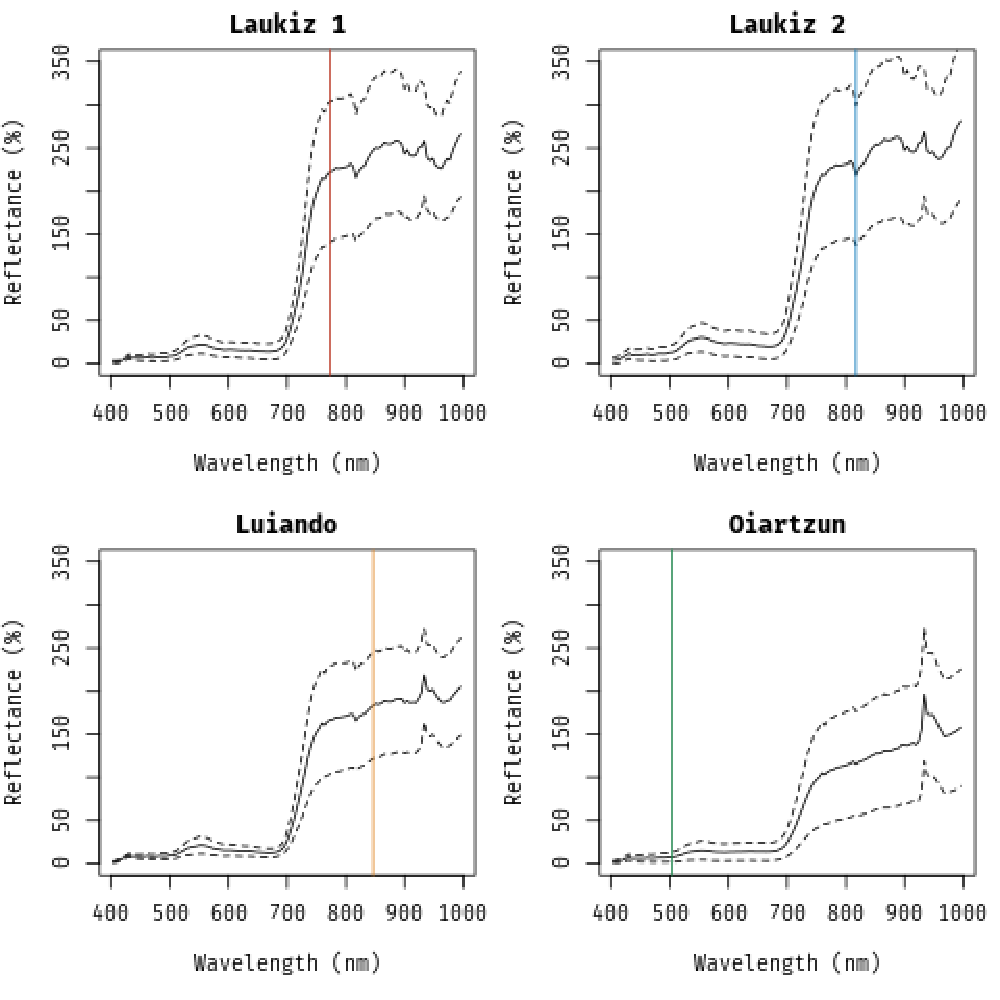
\includegraphics[width=\textwidth] {spectral_signatures.pdf}}
%\caption{Spectral signatures (mean and standard deviation) of each plot.}
%\label{fig:spectral_signatures}
%\end{center}
%\end{figure}

\pagebreak


\section*{References}

\bibliography{Biblio}

\end{document}

